\chapter{Introduction}

{
    With the continuous increase of data and devices in wireless networks, 
existing wireless networks have been facing difficulty to withstand 
increasing traffic load. Consequently, the next generation of mobile 
cellular communication and networking system (5G) has emerged to meet 
these intense demands via innovative technologies, e.g. Network Function 
Virtualization (NFV), Software-Defined Network (SDN), Device-to-Device (D2D) 
communications, etc. Enhanced Mobile Broadband brings 100 times higher 
data rates than that of 4G that can reach 10 gigabits per second. Massive 
Type Communications require a Base Station (BS) to manage an enormous 
number of devices that are designed for Internet of Things (IoT) in general. \\
}


{
    5G is highly flexible and heterogeneous with numerous communication 
    networks involved. According to International Telecommunication Union (ITU),  
    low penetrability of high-frequency signals adopted in 5G and networks 
    consist of a large number of small Access Points (AP) to provide high 
    data access rates and available network bandwidth. \\
}

\section{Handover}
{
    Mobile handover technology, which underpins the continuity of mobile 
    network service, allows ME to move seamlessly between different base 
    stations (BSs) or access points (APs) equipped with different access 
    technologies. Handover or Handoff is an important element in planning and deployment 
    of cellular networks. The deployment of small APs brings frequent 
    horizontal handovers in the cellular network.
}

\newpage
\section{Classification of Handover}
{
    There are many taxonomies to classify handover, for
instance, based on the carrier frequency, handover can be classified
into inter/intra-frequency handover. But according to the proposed solution in chapter 4,
we will talk about Intra/Inter Mobililty Management Entity (MME) handover.
}
\begin{figure}[ht]
    \centering
    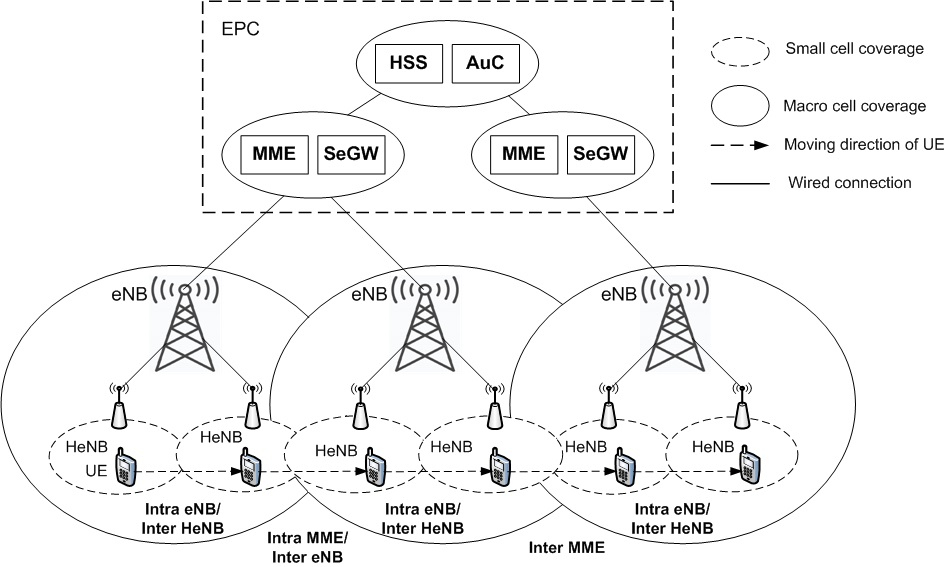
\includegraphics[scale=0.8]{img/handover.jpg}
    \caption{Intra/Inter MME handover}
\end{figure}

\subsection{Inter MME Handover}{
    In this, two MMEs are involved in handover, source MME and target MME.
    The source MME (S-MME) is in charge of the source eNodeB and target MME (T-MME) 
    is in charge of target eNodeB.\\
    Inter MME Handover occur from source eNodeB to target eNodeB.
}

\subsection{Intra MME Handover}{
    In this, only one MMEs is involved in handover.
    The same MME is the charge of the source eNodeB and target eNodeB.\\
    Inter MME Handover occur from source eNodeB to target eNodeB.\\
}


\section{What is blockchain}{
    A blockchain is a distributed database that is shared the 
    various nodes of a laptop community. As a database, a 
    blockchain stores data electronically in digital layout. 
    Blockchains are first-rate known for his or her important 
    position in cryptocurrency structures, such as Bitcoin, 
    for maintaining a relaxed and decentralized record of 
    transactions. The innovation with a blockchain is that it 
    ensures the accuracy and security of a document of records 
    and generates agree with without the need for a trusted 3rd 
    party.\\
}
\begin{figure}[ht]
    \centering
    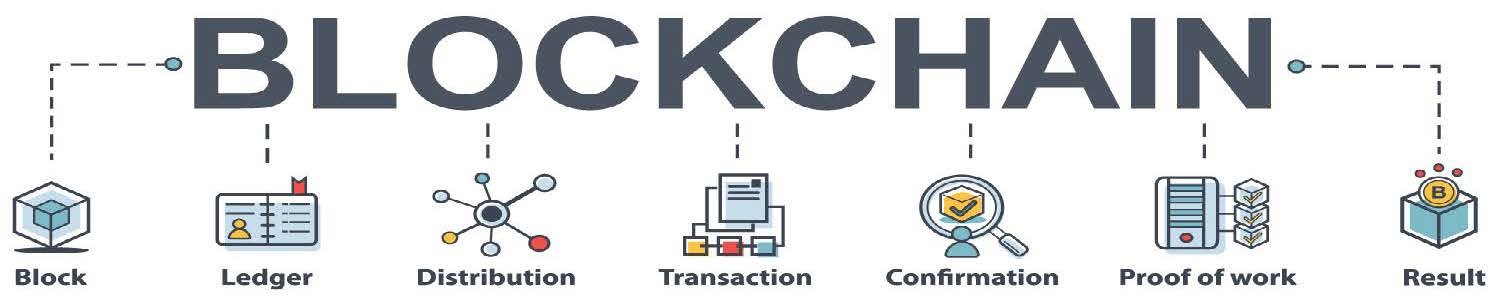
\includegraphics[scale=0.5]{img/blockchain.jpg}
    \caption{Key Component of Blockchain}
\end{figure}

\vspace{1cm}

{
    According to a study, it is proved that cell shrinking and low 
    penetrability of millimeter-wave make the handover happens 
    every 11.6 seconds. So, smoothly supporting mobility among the eNBs 
    is big challenge while maintianing security of the mobile network.\\\\
}
{
    By keeping this concept in mind, I have worked on building a
    network model which is fast and secure enough.
}